\documentclass[prl, reprint, final, showkeys]{revtex4-1}

\usepackage{amsmath}
\usepackage{amsfonts}

\usepackage{graphicx}
\usepackage{subcaption}

\usepackage{epstopdf}

\begin{document}


\title{Characterizing System Dynamics using Diffusion Maps: A Chemotaxis Case Study}

\author{Carmeline J. Dsilva}
\email{cdsilva@princeton.edu}
\affiliation{Department of Chemical and Biological Engineering, Princeton University, Princeton, NJ, 08544}

\author{Ronen Talmon}
\email{ronen.talmon@yale.edu}
\affiliation{Department of Mathematics, Yale University, New Haven, CT, 06520}

\author{Ronald R. Coifman}
\email{coifman@math.yale.edu}
\affiliation{Department of Mathematics, Yale University, New Haven, CT, 06520}

\author{Ioannis G. Kevrekidis}
\email{yannis@princeton.edu}
\affiliation{Department of Chemical and Biological Engineering, Princeton University, Princeton, NJ, 08544}
\affiliation{Program in Applied and Computational Mathematics, Princeton University, Princeton, NJ, 08544}

\date{\today}

\begin{abstract}

Many dynamical systems are governed by stochastic, noisy motions at the microscale which give rise to smooth, coherent dynamics at the macroscale.
%
The relationship between the microscopic and macroscopic dynamics is often not immediately obvious and either requires some modeling assumptions or extensive observation of the system.
%
We demonstrate how extracting macroscopic dynamics from microscale data can be accomplished automatically using manifold learning techniques. 
%
These data-driven algorithms need no {\em a priori} knowledge about the appropriate macroscopic model, but instead, only require the appropriate observers and pairwise metric between observations in order to recover the governing macroscopic variables.
%
We also show how these algorithms can detect changes in the macroscopic dynamical behavior as a function of the microscopic system parameters. 
%
We illustrate these ideas using a model which arises in studies of cellular chemotaxis.

\end{abstract}

\keywords{diffusion maps, earth mover's distance, histograms}

\maketitle

%\section{Introduction} 
 
Often, systems which are stochastic and noisy on the microscale exhibit coherent dynamics on the macroscale which are governed by only a few parameters.
%
For example, fluid flow, which can be described via the position and velocity of every fluid particle, is modeled at the macroscale using the Navier-Stokes equations.
%
However, in general, this mapping from microscale to macroscale is not always obvious.
%
We would like to {\em automatically} uncover a system's macroscale behavior from data collected at the microscale without any {\em a priori} knowledge of the appropriate microscopic or macroscopic model.
%
%TODO: write where this has been done in other places, context, etc.

In this letter, we will present how this goal can be achieved through a data-driven method based on geometric analysis and manifold learning. 
%
Specifically, we aim to emphasize two particular aspects of manifold learning from a dynamical systems' point of view: (a) choosing the appropriate observers, especially in presence of stochastic dynamics, and (b) selecting an appropriate metric for comparison \cite{mallat2012group}. 
%
We will show that both are essential for data-driven algorithms to successfully uncover the underlying system dynamics. 

We will illustrate these points using a model problem which arises in studies of cellular chemotaxis \cite{othmer2000diffusion}.
%
In this example, the macroscopic dynamics vary depending on the value of a single system parameter.
%
We will demonstrate how we can use diffusion maps \cite{coifman2005geometric}, a manifold learning technique, to {\em automatically} detect changes in the system's macroscopic dynamics from microscale data.
%
This case study exhibits several key points which allow us to demonstrate the strength of our approach.
%
First, this system has random microscopic behavior with smooth macroscopic dynamics governed by a single parameter which determines the regime/mode of the system. 
%
Second, it consists of an ensemble of individual stochastic particles which must be described using the appropriate observers.
%
Third, it has an analytic macroscopic description, which serves as a ground truth and will allow us to verify our results which are obtained in an unsupervised manner.
%
We will show that manifold learning algorithms based on statistical observers and with the appropriate affinity metric between pairs of observations uncovers a description of the microscopic data which is consistent with the macroscopic model.
%
Furthermore, these data-driven methods allow us to detect changes in dynamical behavior resulting from changes in the system parameters. 

The remainder of this letter is organized as follows. 
%
We begin by describing the chemotaxis problem, the illustrative example used to demonstrate the methodologies.
%
We present the stochastic microscopic model, and use diffusion maps, a nonlinear dimensionality reduction technique, to analyze microscopic simulation results.
%
We show that the governing macroscopic variables can be recovered, provided that the appropriate observers and distance metric are used.
%
We then describe how, for this example, the microscopic model gives rise to a compact macroscopic description governed by a single parameter, and show that the diffusion maps results are consistent with this macroscopic description. 
%
Finally, we demonstrate that diffusion maps can also identify the relative importance of system variables in different parameter regimes, and detect changes in macroscopic dynamical behavior.

%\section{Problem formulation}

%\subsection{Chemotaxis ``story''} 

Biological cells are one common example of a system where microscopic entities work together and exhibit coherent macroscopic dynamics, in order to to accomplish tasks such as finding food or navigating away from toxins.
%
The cellular dynamics are often governed by extracellular sensed signals; this movement is known as chemotaxis. 
%
Several microscopic models have been proposed to describe chemotaxis dynamics \cite{othmer1988models, codling2008random}.
%
We will analyze one such model described by a one-dimensional velocity jump process \cite{othmer2000diffusion}.
%
In this model, each cell is initialized with a position and a velocity on a line, and the dynamics of each cell are governed by a stochastic process.
%
At random times, a cell will ``turn around'' and switch the direction of its velocity (this turning is controlled by extracellular signals). 
%
%We will analyze the dynamics of collections of such cells/particles. 

%\subsection{Stochastic particles}

The microscopic model consists of a collection of $N$ particles whose states are defined by their positions and velocities. 
%
Let $x_i(t)$ and $v_i(t)$ denote the position and velocity of particle $i$ at time $t$, respectively.
%
The velocity of each particle is either $\pm s$, where $s$ is a (fixed) speed. 
%
We initialize the particles such that
\begin{equation}\label{eqn:system}
\begin{aligned}
x_i(0) & = 0 \\
\mathbb{P} \{ v_i(0) = +s \} & = p
\end{aligned}
\end{equation}
where $p$ is an initial probability.
%
The velocity of each particle randomly switches between $\pm s$ following an (independent) Poisson process with rate $\lambda$.
%

This particular example has an analytic macroscopic equation that governs the overall system behavior.
%
For a large collection of particles ($N \rightarrow \infty$), the system can be described by the probability density of the particles.
%
Let $\rho(x, t)$ denote the probability density of the particles, and let $\rho^-(x, t)$ and $\rho^+(x, t)$ denote the densities of the particles moving towards the positive and negative axis directions, respectively.
%
It can be shown that, as $N \rightarrow \infty$, the densities obey the following set of partial differential equations (PDEs) \cite{othmer2000diffusion}:
\begin{equation} \label{eqn:coupled_pdes}
\begin{aligned}
\frac{\partial \rho^+}{\partial t} + s \frac{\partial \rho^+}{\partial x} & = -\lambda \rho^+ +\lambda \rho^- \\
\frac{\partial \rho^-}{\partial t} - s \frac{\partial \rho^-}{\partial x} & = \lambda \rho^+ -\lambda \rho^- 
\end{aligned}
\end{equation}
%
Alternatively, \eqref{eqn:coupled_pdes} can be rewritten as one, second--order PDE:
\begin{equation} \label{eq:second_order_pde}
\frac{\partial^2 \rho}{\partial t^2} + 2 \lambda \frac{\partial \rho}{\partial t} = s^2 \frac{\partial ^2 \rho}{\partial x^2}
\end{equation}
%
%We assume that $s^2/\lambda = D$ is constant, so that the dynamics of the probability density are governed by a {\em single} parameter $\lambda$.
%
For fixed values of $\lambda$ and $s$, the macroscopic state of the system (the probability density of the particles) is a function of two independent variables: $p$, which controls the initial distribution of the particles, and $t$, the time. 
%
This implies that for fixed $\lambda$ and $s$, the {\em microscopic} data which lie in a high-dimensional ambient space (e.g., the positions of all $N$ particles) should lie on a two-dimensional manifold parameterized by $p$ and $t$, 
so that uncovering the low-dimensional structure reveals the governing macroscopic variables.

We consider two asymptotic regimes of simulation.
%
When $\lambda \rightarrow 0$, the right-hand side of \eqref{eqn:coupled_pdes} tends to 0, and \eqref{eqn:coupled_pdes} becomes two uncoupled wave equations,
\begin{equation}
\begin{aligned}
\frac{\partial \rho^+}{\partial t} + s \frac{\partial \rho^+}{\partial x} & = 0 \\
\frac{\partial \rho^-}{\partial t} - s \frac{\partial \rho^-}{\partial x} & = 0.
\end{aligned}
\end{equation}
%alternatively, \eqref{eq:second_order_pde} becomes the second order wave equation,
%\begin{equation}
%\frac{\partial^2 \rho}{\partial t^2} = s^2 \frac{\partial ^2 \rho}{\partial x^2}.
%\end{equation}

%Dividing \eqref{eq:second_order_pde} by $\lambda > 0$ yields
%\[
%\frac{1}{\lambda} \frac{\partial^2 \rho}{\partial t^2} + 2 \frac{\partial \rho}{\partial t} = D \frac{\partial ^2 \rho}{\partial x^2}
%\]
When $\lambda \rightarrow \infty$, \eqref{eq:second_order_pde} approaches the heat equation,
\begin{equation}
2 \frac{\partial \rho}{\partial t} = D \frac{\partial ^2 \rho}{\partial x^2}.
\end{equation}
%
%Two variables determine the macroscopic state of the system: the initial distribution, which is controlled by a single parameter $p$, and the time, $t$.
%
The above analysis shows that the initial distribution of velocities of the particles (determined by $p$ in the microscopic simulations) plays a very different role depending on the value of $\lambda$.
%
When $\lambda \rightarrow 0$, the dynamics are described by two wave equations, and the initial distribution persists throughout the trajectory.
%
When $\lambda \rightarrow \infty$, the dynamics are described by one heat equation, and the initial conditions are insignificant -- the velocity distribution quickly equilibrates and we see purely diffusive behavior.

For general dynamical systems, the governing macroscopic variables and asymptotic behavior may not be immediately obvious, and instead need to be inferred/identified from the data.
%
We expect the simulation data to lie on a low-dimensional manifold which is parameterized by the macroscopic variables.
%
We use diffusion maps \cite{coifman2005geometric}, which is a manifold learning technique, to uncover such low-dimensional structure and to analyze the results of our microscopic chemotaxis simulations.
%
Compared to principal components analysis (PCA) \cite{...}, a standard linear technique, diffusion maps provides a parameterization of data which lie on a low-dimensional, (possibly) {\em nonlinear} structure in a high-dimensional space.
%
Diffusion maps is simply one of many recently introduced manifold learning techniques that could be used to analyzed the data \cite{...}.

\begin{figure*}[t!]
\def\figwidth{6.4cm}
\begin{subfigure}{\figwidth}
\includegraphics[width=\textwidth]{EMD_withhist_p_1}
\caption{}
\label{subfig:small_lambda_p}
\end{subfigure}
\begin{subfigure}{\figwidth}
\includegraphics[width=\textwidth]{EMD_withhist_t_1}
\caption{}
\label{subfig:small_lambda_t}
\end{subfigure}
\begin{subfigure}{\figwidth}
\includegraphics[width=\textwidth]{EMD_withhist_p_400}
\caption{}
\label{subfig:large_lambda_p}
\end{subfigure}
\begin{subfigure}{\figwidth}
\includegraphics[width=\textwidth]{EMD_withhist_t_400}
\caption{}
\label{subfig:large_lambda_t}
\end{subfigure}
\caption{Diffusion maps embeddings computed from simulation data of the velocity jump process with (a,b) $\lambda=1$, $s=1$, and (c,d) $\lambda=400$, $s=20$.  For each set, we run many simulations, each with $N=1000$ particles.
%
We vary the initial conditions such that $0.1 \le p  \le 0.9$, and allow each simulation to evolve for $10$ time units.
%
We discard the initial portion of each simulation trajectory corresponding to $t < 1$, as it tends to be very noisy and corresponds to initial relaxation of the system.
%
The observations $z(i) \in \mathbb{R}^n$ are the histogram of $x_1(i), x_2(i), \dots, x_N(i)$ into $n =32$ bins.
%
The distances used in the diffusion maps kernel are the earth mover's distances between the histograms of particle positions. The data are colored by (a, c) $p$, the initial probability of a particle moving to the right, and (b, d) $t$, time. Representative histograms are shown for selected data points.}
\label{fig:dmaps_embed_emd}
\end{figure*}

In general, manifold learning techniques have two essential components.
%
One is the appropriate {\em observers} of the system. 
%
These observers should be informative as to the state of the system, as well as invariant to noise in the system. 
%
Two is a {\em distance metric} between the observations that captures a notion of locality: observations which we percieve to be similar should have a small distance. 

Let $z(t) \in \mathbb{R}^n$ denote an $n$-dimensional observation of the system at time $t$. 
%
For the chemotaxis example, we use histograms of the particle positions as observers \cite{talmon2013empirical}. 
%
Histograms are invariant to the indexing of the particles, while retaining the spatial locations of the particles.
%
Instead of the standard Euclidean metric, we use the earth mover's distance (EMD) \cite{rubner2000earth} as the metric between pairs of histograms. 
%
Conceptually, EMD measures how much ``work'' it takes to transform one probability density into another.
%
It therefore not only considers where the densities are inconsistent, but also how far apart the inconsistencies are.
%
Although the brute-force computation of the EMD is computationally expensive, there has been a plethora of work in developing efficient algorithms for the computation of EMD \cite{Pele-eccv2008, Pele-iccv2009}.
%
%TODO: we need to pay a special attention to the implementation of the EMD. We need to make it cleat that this distance can be very efficiently implemented  and therefore it is suitable for the practical uses and algorithm that we propose here as a viable tool for dynamical system analysis.
%
For the special case of one-dimensional data, the EMD is equivalent to the $L_1$-norm between the cumulative distribution functions \cite{rubner2000perceptual}, which can be estimated from histograms as
\begin{equation}
\| z(i) - z(j) \|_{EMD} \approx \sum_{l=1}^{n} \left| \sum_{k=1}^l z_k(i) - \sum_{k=1}^l z_k(j) \right|
\end{equation}
where the histograms $z(i), z(j)$ are defined on equally-spaced bins in $\mathbb{R}$. 

Assume we are given $m$ observations $z(1), \dots, z(m)$, which lie on a $d$-dimensional, nonlinear manifold, with $d \ll n$. 
%
%TODO: add a couple of sentences to relate the notion of manifolds and parameterization to the dynamical system setup. Possibly use PCA reference.
Our goal is to uncover a $d$-dimensional parameterization of the $m$ observations that respects the underlying manifold geometry.
%
We first construct the matrix $W \in \mathbb{R}^{m \times m}$, with
\begin{equation} \label{eq:W}
W_{ij} = \exp \left( -\frac{\|z(i) - z(j) \|^2}{\epsilon^2} \right), \ i,j=1,\ldots,m
\end{equation}
where $\| \cdot \|$ denotes the appropriate norm for the data, and $\epsilon$ is a characteristic distance between the observations. 
%
For the chemotaxis example, we use the EMD as the norm, and we take $\epsilon$ to be the median of the pairwise distances between the data points.
%
We then construct the diagonal matrix $D \in \mathbb{R}^{m \times m}$, with $D_{ii} = \sum_j W_{ij}$, and the matrix $A  = D^{-1} W.$
%
The eigenvectors $\phi_0, \phi_1, \dots, \phi_{m-1}$ of $A$ then provide the embedding coordinates for the data, such that
$\phi_{j}(i)$ is the $j^{th}$ embedding coordinate for $z(i)$.
%
The ``importance'' of coordinate $\phi_j$ is quantified by the corresponding eigenvalue $\mu_j$, e.g. the relative importance of $\phi_1$ versus $\phi_2$ can be measured by comparing $\mu_1$ and $\mu_2$.
%
We order the eigenvectors such that $|\mu_0| \ge |\mu_1| \ge \dots \ge |\mu_{m-1}|$, and if the data are low-dimensional, we only need to retain a few of the leading eigenvectors to adequately describe the data.
%
Because the matrix $A$ is row-stochastic ($\sum_j A_{ij} = 1$),  $\mu_0 = 1$ and $\phi_0$ is a constant vector which is not used as an embedding coordinate.

Figure~\ref{fig:dmaps_embed_emd} shows the results of analyzing two sets of chemotaxis simulations using diffusion maps. 
%
One set of simulations (Figures~\ref{subfig:small_lambda_p}~and~\ref{subfig:small_lambda_t}) is for a small value of $\lambda$, and the other set (Figures~\ref{subfig:large_lambda_p}~and~\ref{subfig:large_lambda_t}) is for a large value of $\lambda$. 
%
For both sets of simulations, the two macroscopic variables, $p$ and $t$, are well-correlated with the first two diffusion maps coordinates, $\phi_1$ and $\phi_2$. 
%
In both cases, $\phi_1$ is significantly more important than $\phi_2$, indicated by the separation between the first two eigenvalues (for the small $\lambda$ case, $\mu_1 = 0.5138$, and $\mu_2 = 0.3943$, and for the large $\lambda$ case, $\mu_1 = 0.5543$, and $\mu_2 = 0.3807$).
%
$\phi_1$, the ``more important'' coordinate, is correlated with $p$ for the small $\lambda$ case (Figure~\ref{subfig:small_lambda_p}), and correlated with $t$ for the large $\lambda$ case (Figure~\ref{subfig:large_lambda_t}), indicating that the relative importance of $p$ and $t$ changes in the two simulations;
this is consistent with the analytic macroscopic description. 
%
Furthermore, in the small $\lambda$ regime (wave equation), shown in Figures \ref{subfig:small_lambda_p} and \ref{subfig:small_lambda_t}, the points corresponding to small times are more tightly clustered than the points corresponding to large times.
%
This is consistent with the macroscopic model: at small times, the particles are more condensed around $x=0$, and it is more difficult to distinguish the particles moving to the left from the particles moving to the right. 
%
On the other hand, at large times, once the particles evolve from the origin, this separation is clear.  
%
For the large $\lambda$ case (heat equation), shown in Figures \ref{subfig:large_lambda_p} and \ref{subfig:large_lambda_t}, we observe that at small times, the initial distribution $p$ is well organized in the embedding in Figure \ref{subfig:large_lambda_p}, as the velocity distribution of the particles is initially skewed and can be seen in the initial displacements 
%
On the other hand, for large times, we observe that the initial distribution $p$ is less organized in Figure \ref{subfig:large_lambda_p}, as the velocities have equilibrated and the initial distribution is less detectable in the particle density.


%correlations
%small lambda
%Euclidean: 3.3848e-04, -0.1861
%EMD: 0.9000, 0.9807
 %   
%large lambda
%Euclidean: -0.5466, 0.3329
%EMD: 0.9329, 0.9832

To emphasize the importance of using the correct distance metric, we also computed the diffusion maps embeddings of the two sets of simulation data, using the standard Euclidean distance between the histograms to compute the distances in \eqref{eq:W}.
%
There is no appreciable correlation between the embedding coordinates and the macroscopic variables $p$ and $t$ (the correlations between the embedding coordinates and the macroscopic variables are all  less than 60\%, with the correlations for the small $\lambda$ case being less than 20\%). 
%
This is due to the inappropriate metric, which does not accurately describe the distances between histograms.
%
In contrast, the correlations between the embedding coordinates and the macroscopic variables when using EMD in the diffusion maps calculation are all greater than 90\%.



\begin{figure}[t] 
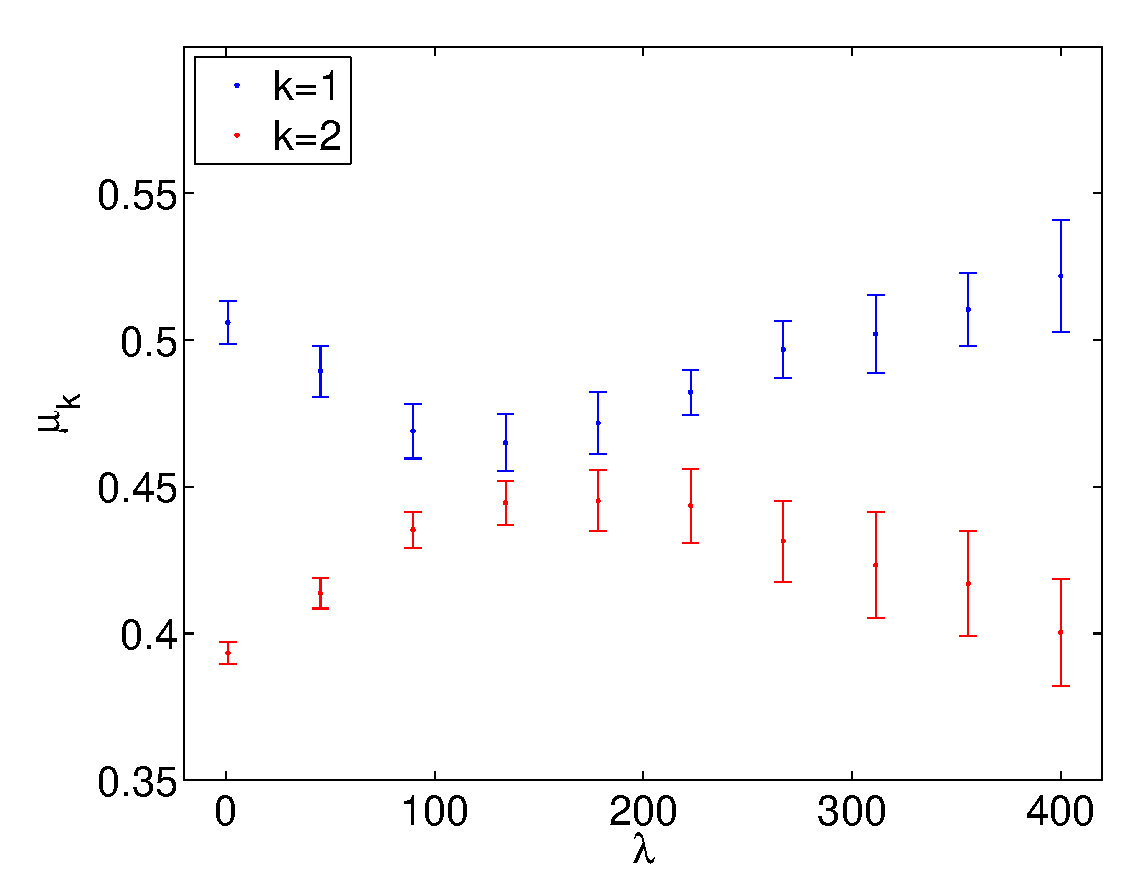
\includegraphics[width=8cm]{detect_change_eigenvalues}
\caption{The first two eigenvalues from DMAPS as a function of $\lambda$. Each point is averaged over 10 simulation experiments (as in Figure~\ref{fig:dmaps_embed_emd}, one experiment consists of data collected at varying $p$ and $t$, for a fixed value of $\lambda$), with error bars indicating one standard deviation. 
The convergence of the eigenvalues at $\lambda \approx 125$ indicates switching of the dynamical ``mode'' of the system.}
\label{fig:detect_change}
\end{figure}

We have seen that the eigenvalues $\mu_i$, which quantify the importance of each embedding coordinate, reveal the relative importance of the variables which govern the macroscopic dynamics.
%
We can also use these eigenvalues to detect the change in dynamical behavior.
%
We showed that at the two asymptotic regimes ($\lambda \rightarrow 0$ and $\lambda \rightarrow \infty$), there is a gap between the two eigenvalues, as one of the macroscopic variables is significantly more important to the dynamical behavior.
%
For intermediate $\lambda$ values, we expect the gap between $|\mu_1|$ and $|\mu_2|$ to narrow, and that the $\lambda$ value where $|\mu_1| \approx |\mu_2|$ corresponds to the transition between ``wave-like'' and ``heat-like'' behavior. 

To demonstrate this point, we performed a new set of experiments, where we simulated the dynamical system over a range of $\lambda$ values. 
% 
Figure~\ref{fig:detect_change} shows the first two diffusion maps eigenvalues, $\mu_1$ and $\mu_2$, computed from these simulations, as a function of $\lambda$.
% 
%TODO: describe as a new experiment with a new data set. The goal of this experiment is to show implicit data-driven phase shift detection.
%
For small $\lambda$ (the wave-equation regime, corresponding to Figures~\ref{subfig:small_lambda_p}~and~\ref{subfig:small_lambda_t}), the two eigenvalues are well-separated, as the first mode (which parameterizes $p$) is significantly more important than the second mode (which parameterizes $t$).
%
At intermediate $\lambda$ values, the eigenvalues come together as the system dynamics change and both $p$ and $t$ are of similar importance.
%
The eigenvalues then separate again at large $\lambda$ (the heat equation regime, corresponding to Figures~\ref{subfig:large_lambda_p}~and~\ref{subfig:large_lambda_t}), where the $t$ effects dominate the dynamics.
%
We can therefore detect where the change in dynamical behavior occurs using data-driven techniques, without any knowledge of the governing macroscopic model. 

%\begin{figure}[t]
%\def\figwidth{4.2cm}
%\begin{subfigure}{\figwidth}
%\includegraphics[width=\textwidth]{rawhist_p_1}
%\caption{}
%\end{subfigure}
%\begin{subfigure}{\figwidth}
%\includegraphics[width=\textwidth]{rawhist_t_1}
%\caption{}
%\end{subfigure}
%\begin{subfigure}{\figwidth}
%\includegraphics[width=\textwidth]{rawhist_p_400}
%\caption{}
%\end{subfigure}
%\begin{subfigure}{\figwidth}
%\includegraphics[width=\textwidth]{rawhist_t_400}
%\caption{}
%\end{subfigure}
%\caption{Diffusion maps embeddings computed from simulation data of the velocity jump process with (a,b) $\lambda=1$, $s=1$, and (c,d) $\lambda=400$, $s=20$. The distances used in the diffusion maps kernel are the Euclidean distances between the histograms of particle positions. The data are colored by (a, c) $p$, the initial probability of a particle moving to the right, and (b, d) $t$, time.}
%\label{fig:dmaps_embed_noemd}
%\end{figure}

This paper aims to bridge the fields of data mining and dynamical systems. 
%
For data mining methods to be informative, processing the appropriate statistical moments or observables instead of individual particles/realizations is essential. 
%
In addition, one must also define the appropriate distance metric between the observations.
%
These two components induce the ``correct" Riemannian geometry and allow for informative analyses, such as meaningful and compact parameterization, phase shift detection, and dynamical characterization, through manifold learning.
%
In this paper, these concepts were demonstrated using a dynamical model of cellular chemotaxis with a known analytic macroscopic behavior.
%
We showed that, using histograms as observers and EMD as a distance metric, diffusion maps can uncover the underlying macroscopic dynamical behavior which is consistent with the analytic macroscopic model.
%
We are confident that such techniques can help inform modeling efforts for systems where the macroscopic dynamics and behavior are not currently known. 




%\section{Discussion}


\bibliography{../../references/references}

\end{document}